\documentclass[12pt]{article}
%\VignetteIndexEntry{pmg}
%\vignettepackage{pmg}

\usepackage{times}              % for fonts
\usepackage[]{geometry}
\usepackage{mathptm}            % for math fonts type 1
\usepackage{graphicx}           % for graphics files
\usepackage{floatflt}           % for ``floating boxes''
%%\usepackage{index}
\usepackage{relsize}            % for relative size fonts
\usepackage{amsmath}            % for amslatex stuff
\usepackage{amsfonts}           % for amsfonts
\usepackage{url}                % for \url,
\usepackage{color}
\usepackage{fancyvrb}
\usepackage{fancyhdr}

%% fill these in
\renewcommand{\lfoot}{p m g}
\renewcommand{\rfoot}{page \thepage}
\renewcommand{\headrulewidth}{0.0pt}
\renewcommand{\footrulewidth}{0.1pt}


%% My abbreviations
\newcommand{\RCode}[1]{\texttt{#1}}
\newcommand{\RFunc}[1]{\texttt{#1()}}
\newcommand{\RPackage}[1]{\textbf{#1}}
\newcommand{\RArg}[1]{\texttt{#1=}}
\newcommand{\RListel}[1]{\texttt{\$#1}}


\newenvironment{RArgs}{\begin{list}{}{}}{\end{list}}




\usepackage{/home/verzani/R/lib/R/share/texmf/Sweave}
\begin{document}
\title{pmg}
\author{John Verzani\\\url{pmgRgui@gmail.com}}
\maketitle

\section*{Abstract:}

The \RCode{pmg} package provides a simple GUI for R using the GTK2
toolkit. the \RCode{pmg} GUI is similar in intent to the more mature
\RCode{Rcmdr} GUI which uses the \RCode{tcltk} toolkit. The package
was designed to lessen R's learning curve for students in introductory
course. The GTK libraries are accessed through the \RCode{RGtk2}
package of Michael Lawrence. This package is available for all three
major platforms: windows, Mac OS X, and Unix/X11.  the
\RCode{gWidgets} interface is used to simplify the development of
interactive GUIS, this in turn requires the \RCode{gWidgetsRGtk2}
package.~\footnote{In theory, but not practice, the usage of
  \RCode{gWidgets} would allow \RCode{pmg} to use a different GUI
  toolkit, the \RCode{gWidgetsrJava} package does not have enough
  features in it currently to do so.}


\section{Installing pmg}
If the requisite packages are available on CRAN, then installation can
be done with a single command such as
\begin{Soutput}
> install.packages("pmg", dependencies=TRUE)
\end{Soutput}
or from the toolbar. Mac users may need to add \RCode{source=TRUE}.


The above assumes that both the GTK libraries, the \RCode{RGtk2}
package, and the \RCode{cairoDevice} package already exist on your
system. If not, the home page for \RCode{RGtk2} has some directions
(\url{http://www.ggobi.org/rgtk2}).

For users of windows, a script is available to download the gtk
libraries and install \RCode{pmg}. Run the command
\begin{Sinput}
> source("http://www.math.csi.cuny.edu/pmg/installpmg.R")
\end{Sinput}
to initiate the script.

For users with the \RCode{iplots} or \RCode{reshape} packages
installed, there are extra dialogs appearing under the menu bar.

\section{Starting}

The GUI uses the \RPackage{gWidgets} API. The \RPackage{gWidgets}
package offers the promise of a toolkit-independent API for writing
interactive GUIs. If more than one toolkit implementation is
installed, a menu for selection will be shown. It is likely that
\RPackage{pmg} will only work well using the \RPackage{gWidgetsRGtk2}
implementation

The GUI is started as follows.
\begin{Soutput}
> library(pmg)
\end{Soutput}

To restart the GUI, the command \RFunc{pmg} can be issued. With the
Windows operating system it is best to minimize the parent R GUI as it
covers up the pmg windows.

\section{Using the GUI}

\begin{figure}[htbp]
  \centering
  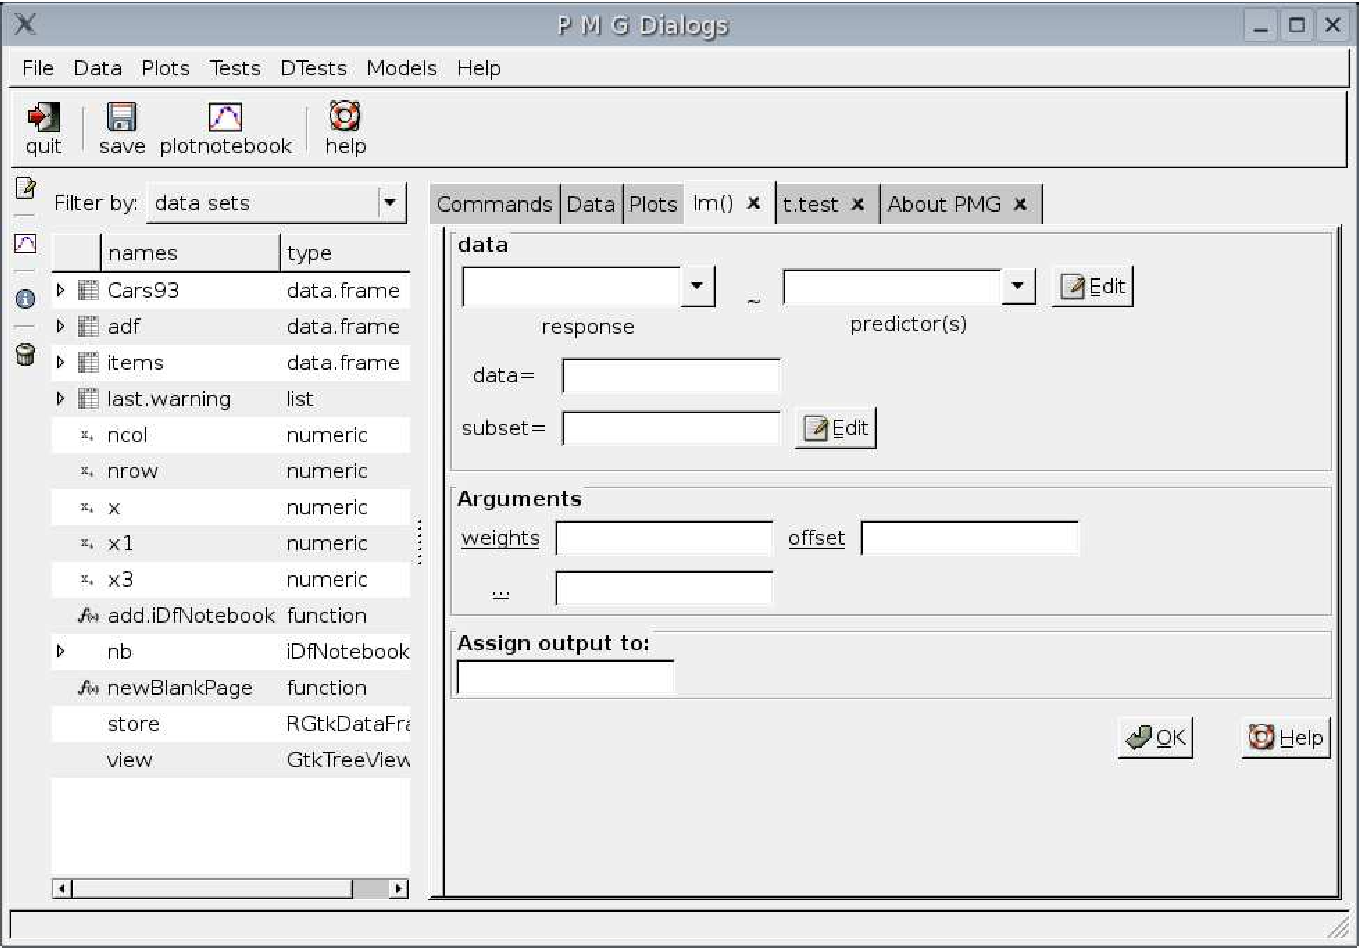
\includegraphics[width=.8\textwidth]{pmg-sample-dialog}
  \caption{The pmg gui with sample dialog}
  \label{fig:pmg-gui-sample-dialog}
\end{figure}


The GUI basically consists of a variable browser and a collection of
dialogs that are accessed through a menubar. The values in the
variable browser may be dragged and dropped into the entry areas of
the dialogs. 

Most of the dialogs have a common format familiar to web users: you
enter in the values in a form and click ``OK.'' The output is then
sent to the console and the ``Commands'' tab.

Besides the menubar, the GUI has a few key features. From left to
right these are:
\begin{description}
\item[Some drop targets on the left hand side] These are for editing the
  dropped object, for plotting the dropped object, for summarizing the
  drop object, or for deleting the dropped object.
\item[The variable browser] This shows the variables in the global
  environment using a familiar tree interface. The filter tab allows
  you to display just some desired types. The definitions of which may
  not be as inclusive as you would like. The base objects are
  refreshed every few seconds. Unfortunately, their subobjects are
  not. To refresh the subobjects, close then open the sub display.

  These variables may be dragged and dropped. For instance, dropping
  on the left sidebar produces the actions described previously.

  If the variables are double-clicked a summary of the object appears
  in a tab in the dialog notebook on the right.
\item[The dialog notebook] This notebook (a widget with tabbed pages)
  has two permanent tabs: a command line and a data frame
  viewer/editor. Other dialogs have a close button in the tab that
  removes that dialog.

  The tabs have a drag motion set so that if an object is dragged over
  the tab, the corresponding page opens.
\item[The ``Commands'' tab]  The command line has two states: one for
  editing the current command, and one for viewing the command with
  its output. Toggling between is done with the buttons immediately
  above the display. The command line processes chunks of R code,
  in the style of sourcing a .R file. A history of the last 25
  commands issued is available. 

  Dragging variables to the command line drops their name into the window.
\item[The dataframe viewer/editor] The dataframe viewer
  (Figure~\ref{fig:pmg-gui-pmg-dataviewer}) allows one to
  view and edit data frames. It should look more spreadsheet like, but
  no such widget is available in GTK. This implementation allows you
  to edit single cells in the table, and edit row and column names. 

  Editing is a little clunky. Double clicking on a cell should allow
  you to edit it. Hitting the enter key, jumps to the next row done
  and opens the edit area. To move to another column use the mouse or
  the arrows and the enter key.
  
  A right-mouse popup menu allows for sorting by column
  values, applying a function to a column, or changing the column
  name. This popup is not bound to the column header, but rather the
  column contents. Click once in a column, then right click to see it.

  A right-mouse popup on the notebook tab holding the name allows you to save, close,
  or rename the sheet.

  The sheets with the names \verb+*scratch:#*+ are treated
  differently. The non-empty individual columns are saved as data
  vectors. Otherwise a saved sheet is saved  as a data frame.

  Dropping an appropriate variable on the open button will open a new tab
  with that variable's contents displayed. Whereas, clicking the open
  button opens a dialog allowing the selection of a data frame.

  
\item[Dialogs] 
  Most of the menu items create dialogs that are attached as notebook
  pages to the right of the data frame viewer/editor. 
  
  There are primarily two types of dialogs in pmg: static ones and
  ``dynamic'' ones. The latter have menu items prefaced with an
  ``execute'' icon, and appear in separate windows. These dynamic
  dialogs were inspired by the Fathom software package
  (\url{http://www.keypress.com/fathom/}).
  
  Dynamic dialogs respond to drag and drop actions. By dragging
  variables onto the appropriate area, the values in the widget get
  updated. Additionally, the bold face values in the widget can be
  clicked to effect changes. Again, the widget refreshes instantly.
  These dynamic dialogs give immediate feedback, but do not show or
  allow one to edit the R commands that are used.

  There are currently 4 main dynamic dialogs: one for exploring
  graphically (the Lattice Explorer), one for finding numeric
  summaries, one for significance tests, and one for linear models.
  

  The static dialogs are illustrated by the sample dialog appearing in
  Figure~\ref{fig:pmg-gui-sample-dialog}. Most, but not all, of the dialogs
  have the same behavior described below. There are areas to enter
  information, and when enough values are specified, the ``ok'' button
  sends the appropriate command to the ``Commands'' tab area to be evaluated.
  Unlike the dynamic dialogs, the value is only updated when the
  ``ok'' button is clicked.  Empty values are ignored. Values may
  need to be quoted. 

 

  
  This particular dialog in Figure~\ref{fig:pmg-gui-sample-dialog}
  expects a model formula, in this case for calling the \RFunc{plot}
  function.

  There are some conveniences for editing the information. When a data
  set is dropped onto the \verb+data=+ area the names of the data
  frame are added to the dropdown values for the response and
  predictor. Additionally, the ``edit'' button opens a dialog for
  editing the formula. A similar button allows one to subset the data
  frame.

  The ``arguments'' section of the dialog has underlined labels. When
  these are clicked the appropriate help page section for this
  argument is looked for and displayed if found (this involves a grep
  for the colon following the argument and may miss). In this dialog, the
  help page refers to that for \verb+plot()+, but the arguments are
  not found. The ``help'' button will show the full help page.

  When  the ``ok'' button is pressed, the arguments are collected and
  pasted together to make a function call. This is then sent to the
  command area and evaluated. To see the output, you need to click the
  command tab. As well, the command and output is printed into the
  console. 
\end{description}

\begin{figure}[htbp]
  \centering
  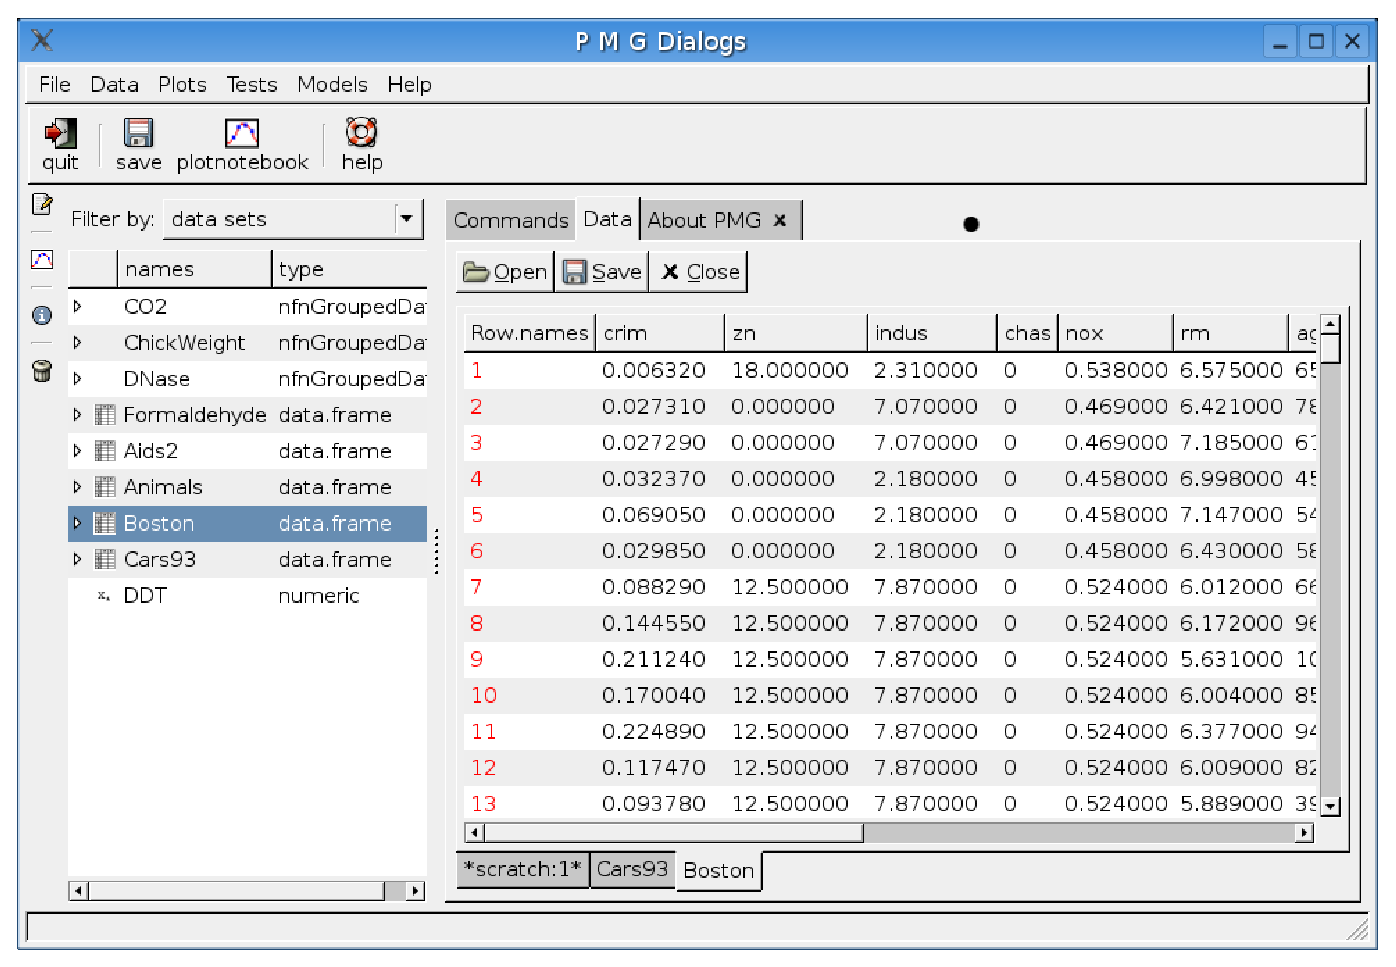
\includegraphics[width=.8\textwidth]{pmg-dataviewer}
  \caption{The data viewer and editor. The columns may be dropped onto
  the dynamic dialogs.}
  \label{fig:pmg-gui-pmg-dataviewer}
\end{figure}


Dialogs are accessed through the menubar. In addition to several of
the ``generic'' dialogs described above, there are some that have
their own window. For example to load a data set so that it is visible
in the variable browser the ``Load data set...''  menu item opens up a
dialog for this. Other dialogs are available for loading an installed
package, installing a package from  CRAN, sourcing a file, saving a
file, etc.


\begin{figure}[htb]
  \centering
  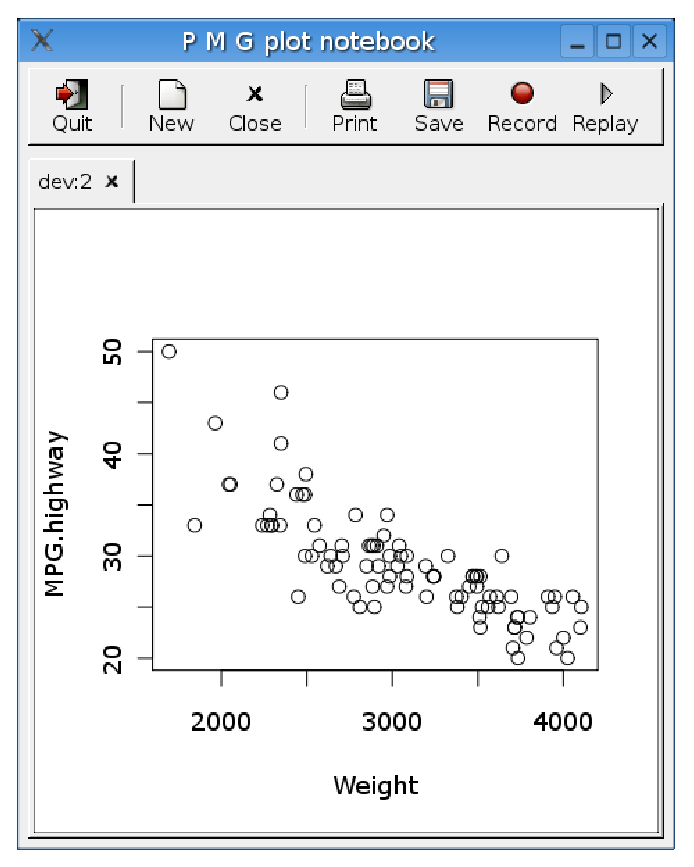
\includegraphics[width=.5\textwidth]{pmg-plotnotebook}
  \caption{A notebook for holding multiple plot devices}
  \label{fig:pmg-gui-plotnotebook-dialog}
\end{figure}



The dialog from ``Data::Univariate Summaries::quantile'' is new as of
version 0.9-24. It is a possible prototype for some student-friendly
dialogs along the lines of the dynamic summaries dialog. For students
there is also a collection of teaching demos under the ``Plots''
menu. 

Graphs can be handled by the default device, through the plot notebook
(Figure~\ref{fig:pmg-gui-plotnotebook-dialog}) which is opened when
the ``plotnotebook'' toolbar item is pressed, or using the Lattice
Explorer. The notebook allows one to store several different plots at
once. The currently selected tab, should also be the current device.
(Using both the plot notebook and the Lattice Explorer can lead to
confusion, as the current device is where the new figure is drawn, and
this may not be the desired device.)

The ``help'' toolbar item opens up a help page browser, allowing
access to R's help system. 


\section{A few sample tasks}

We describe how to perform a few common tasks from an introductory
statistics course.

\subsection{Loading a data set and using a boxplot to explore a
  variable}

Let's see how to make boxplots of the \RCode{MPG.highway} variable
broken up by the number of \RCode{Cylinders} in the data set
\RCode{Cars93} of the \RCode{MASS} package. The first task is to load
the data set. Of course, you might think:
\begin{Soutput}
> library(MASS); boxplot(MPG.highway ~ Cylinders, Cars93)
\end{Soutput}
but we are interested in doing this through the GUI.

First we load the \RCode{MASS} package using the ``Load package''
dialog under the File menu. Open the dialog, and then double click on
MASS until the second column says TRUE.

Next, we call \RCode{data} on the data set so that it appears in the
variable browser. Open the ``Load data set...'' dialog under the Data
menu. Find the data set and then double click. The data set should
appear in the variable browser shortly.

Now open the Lattice Explorer dialog under the Plots menu. Change the
plot selection to \RCode{bwplot}. Then in this order drag the
\RCode{MPG.highway} variable and then the \RCode{Cylinders} variable
onto the main explorer area. The appropriate graph should be
drawn. The basic idea is that the first variable is split up by the
second, and in this case a third is possible. (Drop \RCode{Origin} to
see.)

To look at new variables clear out the old ones with the clear
button. To make a different graphic with the same variables, you only
need to change the graph selection popup.


\subsection{Using the subset feature of the data viewer}

An alternative approach to using lattice graphics to break up the data
by levels of some factor can be to use the \RCode{subset=} dialog for
the data viewer. Changing the values shown in the data viewer, can
dynamically update the graphic. 

To illustrate, open the Lattice Explorer as before and change the plot
selection to \RCode{bwplot}. Now drag the variable \RCode{Cars93} from
the variable browser area \textit{over} the Data tab of the dialogs
area (to open up that tab) and drop the \RCode{Cars93} variable onto
the area where a data frame is shown. This should cause the data
viewer to open and display the data frame. Now drag the
\RCode{MPG.highway} variable name (the column header) onto the Lattice
Explorer dialog and drop it in the graphing area. A boxplot of the
variable is drawn. This boxplot is linked to the values displayed in
the \RCode{MPG.highway} column. Changing a value causes the graphic to
be redisplayed taking into account the new values. We will change the
values with the \RCode{subset=} dialog. At the bottom of the data
viewer is an expander group that must be clicked to show the dialog.
After this appears, you can select a variable and a subsetting
argument to filter the displayed values.
Figure~\ref{fig:data-viewer-with-subset} shows the dialog with only
the 3 cylinder cars shown.

\begin{figure}[htbp]
  \centering
  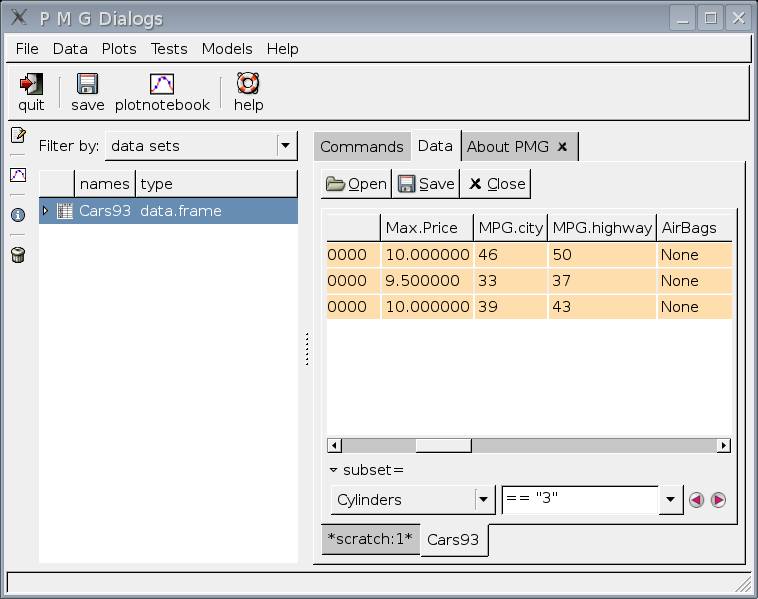
\includegraphics{data-viewer-with-subset}
  \caption{Data viewer showing \RCode{Cars93} data set subsetted by the number of \RCode{Cylinders} being 3.}
  \label{fig:data-viewer-with-subset}
\end{figure}

If you scroll through the levels of \RCode{Cylinder} using the arrow
keys, the boxplot in the Lattice Explorer will be  redrawn each time
using only the visible data.


Dragging a column header onto a widget only works for the dynamic
widgets and only with \RCode{gWidgetsRGtk2}. There are currently two
other dynamic widgets: one for numeric summaries of a data set and
another for linear models.

\subsection{using \RPackage{iplots}}

If the \RPackage{iplots} package is installed the dialog found under
\RCode{Plots::iplots} can also be used to dynamically adjust a graphic
to a mouse click. To see how the highway mileage varies with the
number of cylinders involves the following steps: open the dialog
under \RCode{Plots::iplots}. Then add the data frame
\RCode{Cars93}. Then select the variable \RCode{MPG.highway} on the
left and then under \RCode{New plot} select the \RCode{ihist}
choice. The histogram is created. Now select the \RCode{Cylinders}
variable, but this time make a bar plot using \RCode{ibar}. Another
graphic is opened. Clicking on one of the bars in the barplot causes
those cases to highlight in the histogram. One can also select cases
by dragging over multiple values of the bar plot.

There are plans for a similar interface to \RPackage{rggobi}.

\subsection{Finding numeric summaries of a data set}
\label{sec:numeric-summaries}

The Dynamic Summaries dialog found under the Data menu allows one to
easily find some common numeric summaries. The interface is intended
to make the simplest cases easy, if more control over the arguments is
needed then the respective functions have an alternative dialog.

We consider again the \RCode{Cars93} data set and its
\RCode{MPG.highway} variable. To find the mean of all the data, drag
this to the bold-faced area ``Drop variable here.'' The mean should be
calculated and appear below. To break up the data by the levels of
some other variable drag that to the ``group by''
area. Figure~\ref{fig:dynamic-summaries} shows the result (after
resizing the window) of breaking the data up by the \RCode{Cylinders}
variable.

\begin{figure}[htbp]
  \centering
  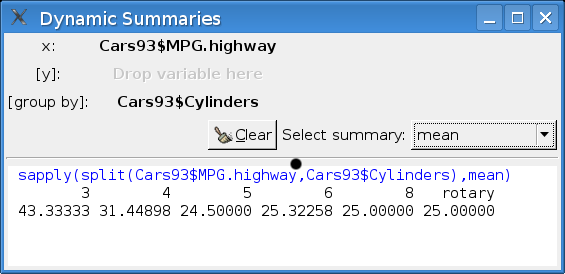
\includegraphics[width=.7\textwidth]{dynamic-summaries}
  \caption{A dialog for computing summaries of numeric data}
  \label{fig:dynamic-summaries}
\end{figure}

Changing the summary using the popup will compute the new numeric
summary. If the variables need to be changed, one can drag a new
variable directly, or if the size is not compatible, clear the
variables first then drag a new variable.

The drop areas can be edited by clicking on the bold text (familiar to
\url{gmail} users). Press enter when done editing. The variable name
can be directly typed in relative to the global environment. Even
simple functions can be applied. One caveat, if the dropped variable
comes from the data frame viewer then editing won't work. However,
editing the data within the data frame viewer should have its changes
instantly propogate.

\section{Adding to the GUI}

Currently there are only a few ways to add to the GUI.

\subsection{Adding a dialog}

The \RCode{pmg.add(widget, label)} function is used to add a dialog to
the main notebook. It will add to the third tab. The widget is some
\RCode{gWidget} instance. It should not already be attached to some
container. For example, this will add a ``hello world'' tab
\begin{Sinput}
> pmg.add(glabel("Hello world"), label="Hi")
\end{Sinput}

\subsection{Creating a dialog to collect a function's arguments}

The \RCode{pmg.gw(lst,title=NULL)} function is used to add a dialog to collect a
function's argument. The function calls \RCode{ggenericwidget} to
create the dialog. The \RCode{lst} argument can be a list, a function
name or a function. In the last two cases the dialog is formed from
looking at the values returned from \RCode{formals()}. The title can
be set or will be guessed if not present.


\subsection{Adding to the menubar}

The \RCode{pmg.addMenubar(menulist,...)} function can be used to add new top-level
entries  to the menu bar. It takes a list that gets passed to
\RCode{gmenu} as its argument. 

For example, a new entry can be defined as follows
\begin{Sinput}
> lst = list()
> lst$MenuEntry$hi$handler = function(h,...) pmg.add(glabel("HelloWorld"), label="Hi")
> lst$MenuEntry$mean$handler = function(h,...) pmg.gw("mean")
> pmg.addMenubar(lst)
\end{Sinput}




User-defined menus can be added when the GUI is started. At startup
pmg looks for a variable \RCode{pmg.user.menu} which if present should
be a list with named components, each again a list as above. See the
help page for \RFunc{gmenu} of \RCode{gWidgets} for more details on
its structure.

\section{TODO}
The pmg GUI could be improved in many ways. A few obvious ones are
\begin{itemize}
\item More ability to customize the GUI. For instance, there is no way
  to change the fonts, there is only a primitive way to change the
  menubar, ...
\item The bulk of the dialogs are pretty basic -- they just collect
  arguments to pass to a function call. Some more dynamic widgets
  would be useful. The dialog for quantiles is meant to be a template
  for some student-friendly dialogs.
\item It would be great to have some sort of report writing tool. The
  new Maple interface or the Mathematica notebook interface might be a
  good choice for interacting with R.
\end{itemize}


\end{document}

%%% Local Variables: 
%%% mode: latex
%%% End: 
